\documentclass{article}

% arxiv-standard packages
\usepackage[preprint]{neurips_2024}   % swap to [final] for camera-ready
\usepackage[utf8]{inputenc}
\usepackage[T1]{fontenc}
\usepackage{hyperref}
\usepackage{url}
\usepackage{booktabs}
\usepackage{amsfonts}
\usepackage{amsmath}
\usepackage{amssymb}
\usepackage{nicefrac}
\usepackage{microtype}
\usepackage{xcolor}
\usepackage{graphicx}
\usepackage{algorithm}
\usepackage{algorithmic}
\usepackage{multirow}
\usepackage{tabularx}

\title{Dynamic Attentional Context Scoping:\\
Agent-Triggered Focus Sessions for\\
Isolated Per-Agent Steering in Multi-Agent LLM Orchestration}

\author{%
  Nickson Patel \\
  \texttt{nicksonpatel@gmail.com} \\
  \texttt{nickson@x-algo.net}
}

\begin{document}
\maketitle

%-----------------------------------------------------------------------
\begin{abstract}
Multi-agent LLM orchestration systems suffer from \emph{context pollution}:
when $N$ concurrent agents compete for the orchestrator's context window,
each agent's task state, partial outputs, and pending questions contaminate
the steering interactions of every other agent, degrading decision quality.
We introduce \textbf{Dynamic Attentional Context Scoping (DACS)}, a
mechanism in which the orchestrator operates in two asymmetric modes.
In \textsc{Registry} mode it holds only lightweight per-agent status
summaries ($\leq 200$ tokens each), remaining responsive to all agents
and the user.
When an agent emits a \textsc{SteeringRequest}, the orchestrator enters
\textsc{Focus}$(a_i)$ mode, injecting the full context of agent $a_i$
while compressing all other agents to their registry entries.
Context isolation is agent-triggered, asymmetric, and deterministic:
the context window contains exactly $F(a_i) + R_{-i}$ during steering,
eliminating cross-agent contamination without requiring context
compression or retrieval.
We evaluate DACS against a flat-context baseline across $N \in \{3, 5,
10\}$ agents, 10 trials per condition (60 runs total).
DACS achieves $90.0$--$96.7\%$ steering accuracy versus $21.0$--$60.0\%$
for the baseline ($p < 0.0001$ by Welch's $t$-test at all $N$).
Wrong-agent contamination drops from $29$--$57\%$ to $4$--$14\%$.
Critically, DACS context size grows sub-linearly with $N$ (561--816
tokens, $\approx\!+25$ tokens per added agent), while the baseline grows
near-linearly (1{,}191--2{,}883 tokens), yielding a context efficiency
ratio of 2.12--3.53$\times$ that increases with scale.
All code and data are released at
\href{https://github.com/nicksonpatel/dacs-agent-focus-mode}{\texttt{github.com/nicksonpatel/dacs-agent-focus-mode}}.
\end{abstract}

%-----------------------------------------------------------------------
\section{Introduction}
\label{sec:intro}

The deployment of LLMs as orchestrators managing multiple parallel agents
has become a practical reality: systems such as Claude Code Agent
Teams~\citep{anthropic2025code}, OpenCode~\citep{opencode2025}, and
production multi-agent platforms~\citep{agentorchestra2025} demonstrate
that complex long-horizon tasks can be decomposed across concurrent
specialized agents.
The common architectural choice is a single LLM instance (the
\emph{orchestrator}) that coordinates all agents, handles user
interaction, and steers individual agents when they reach decision points.

\paragraph{The context pollution problem.}
This architecture introduces a fundamental scaling problem.
When $N$ agents run concurrently, each maintains its own task context:
partial outputs, domain-specific state, pending decisions.
In a flat-context orchestrator, all of these threads compete for space in
a single context window.
When agent $a_i$ requests steering—``should I use BFS or DFS for this
graph traversal?''—the orchestrator's context simultaneously holds $a_j$'s
transformer attention survey, $a_k$'s CSV encoding problem, and so on.
We call this \emph{context pollution}: the systematic contamination of
one agent's steering interaction by irrelevant context from other agents.

The consequences are measurable and severe.
Prior work has documented context pollution in single-agent settings
under tool overload~\citep{adaptorch2025,codedelegator2025}, under
retrieval bloat~\citep{sidequest2025}, and under long conversation
histories~\citep{afm2024,ace2026}.
Our experiments show that in the multi-agent setting, a flat-context
orchestrator's steering accuracy collapses from 60\% at $N=3$ to 21\% at
$N=10$ while baseline contamination rate stays above 29\% throughout.

\paragraph{The DACS mechanism.}
We propose \textbf{Dynamic Attentional Context Scoping (DACS)}, which
solves context pollution through \emph{agent-triggered asymmetric context
isolation}.
DACS introduces two orchestrator modes:

\begin{itemize}
  \item \textbf{\textsc{Registry} mode.} The orchestrator holds only the
  registry $R = \{r_1, \ldots, r_N\}$—one compact status summary per
  agent ($\leq 200$ tokens each).
  It monitors all agents, responds to the user, and queues incoming
  steering requests.

  \item \textbf{\textsc{Focus}$(a_i)$ mode.} When agent $a_i$ emits a
  \textsc{SteeringRequest}, the orchestrator transitions to hold $F(a_i)$
  (the full context of $a_i$: task description, prior steering exchanges,
  current partial output) plus a compressed version of $R_{-i}$
  (registry summaries for all agents except $a_i$).
  The context window contains exactly what is needed to steer $a_i$,
  and nothing from any other agent's task thread.
\end{itemize}

The key properties of DACS that distinguish it from prior context
management approaches are:
\begin{enumerate}
  \item \textbf{Agent-triggered.} Context isolation fires when an agent
  needs it, not on every turn or at task-decomposition time.
  \item \textbf{Asymmetric.} The steered agent gets full fidelity;
  all others get compressed summaries.
  \item \textbf{Exact, not approximate.} No scoring function, no fidelity
  tiering~\citep{afm2024,lemon2025}, no probabilistic compression—the
  context is deterministically constructed as $F(a_i) + R_{-i}$.
  \item \textbf{Sub-linear in $N$.} Focus context size is independent of
  $N$; only the compressed registry grows (by $\approx 25$ tokens per
  additional agent in our experiments).
\end{enumerate}

\paragraph{Contributions.}
\begin{enumerate}
  \item We formally define the DACS mechanism: the \textsc{Registry}/
  \textsc{Focus} state machine, the \textsc{SteeringRequest} protocol,
  and the context builder invariants (\S\ref{sec:mechanism}).
  \item We implement a minimal, fully observable orchestration harness
  ($\sim$300 lines) where every token entering each LLM call is logged,
  enabling strict experimental control (\S\ref{sec:experiments}).
  \item We show that DACS yields large, statistically significant accuracy
  gains at all agent counts tested, with a context efficiency advantage
  that grows with $N$ (\S\ref{sec:results}).
  \item We identify sub-linear context scaling as the mechanism's key
  theoretical property, explain its source, and discuss the conditions
  under which it holds (\S\ref{sec:discussion}).
\end{enumerate}

%-----------------------------------------------------------------------
\section{Related Work}
\label{sec:related}

Context management for LLM agents has been studied at three levels of
granularity: single-agent memory across turns, single-agent tool/retrieval
bloat, and multi-agent orchestration.
DACS addresses a problem at the third level that existing work at the
first two levels does not reach.

\paragraph{Single-turn context compression.}
AFM~\citep{afm2024} assigns per-message fidelity tiers
(Full/Compressed/Placeholder) based on a composite recency-relevance score
and packs messages greedily under a token budget.
It achieves 83.3\% constraint-recall on its benchmark, validating that
structured fidelity management outperforms naive truncation.
ACE~\citep{ace2026} treats the agent's context as an evolving playbook
of itemized bullets with utility counters, using incremental delta updates
to avoid context collapse (they observe a 18{,}282-token context collapsing
to 122 tokens under iterative rewriting, dropping accuracy below the
no-adaptation baseline).
Both AFM and ACE operate within a single agent's context history.
Neither addresses $N$ concurrent agents competing for an orchestrator
context window, and neither models wrong-agent contamination as a failure
mode.

\paragraph{Retrieval and cache bloat.}
SideQuest~\citep{sidequest2025} frames KV cache compression as an
auxiliary task solved by the LRM itself, achieving 65\% peak token
reduction on single-agent deep research tasks.
Lemon Agent~\citep{lemon2025} applies three-tier progressive compression
(full → compressed → summary) to a shared orchestrator context over task
time in an orchestrator-worker system.
Both treat context as a resource to compress; neither introduces asymmetric
isolation triggered by an agent's request.

\paragraph{Context pollution in tool-heavy agents.}
Adaptive Orchestration~\citep{adaptorch2025} identifies context pollution
and attention decay as failure modes in monolithic agents loaded with too
many tools, and proposes spawning specialist sub-agents (DMoE) to offload
capability.
CodeDelegator~\citep{codedelegator2025} separates planner and executor
roles via Ephemeral-Persistent State Separation (EPSS): a persistent
Delegator never receives execution traces; each Coder sub-task starts with
a clean context.
Both solve context pollution \emph{architecturally} (at task decomposition
time) for sequential delegation to one sub-agent at a time.
DACS solves it \emph{dynamically at runtime}, during the steering
interaction itself, for $N$ agents running simultaneously.
The distinction matters: CodeDelegator's Delegator has no mechanism for
handling the case where multiple concurrent Coders simultaneously need
steering.

\paragraph{Multi-agent orchestration context management.}
AOI~\citep{aoi2024} introduces a three-layer memory architecture for
multi-agent IT operations, with a central Context Compressor transforming
raw agent outputs into a compressed cache.
Its Observer agent always holds a compressed aggregate of \emph{all}
agent activity simultaneously—there is no per-agent isolation.
Agents execute and report results; they cannot signal the orchestrator
for steering attention, and wrong-agent contamination is not modelled
(AOI's failure mode is information loss from operational data volume).
AgentOrchestra~\citep{agentorchestra2025} achieves SOTA on GAIA (89.04\%)
via hierarchical delegation: a planning agent routes sub-tasks to
domain-specific sub-agents, bounding the planner's context footprint by
converting global coordination into localized routing decisions.
The paper explicitly notes that flat coordination ``tends to accumulate
irrelevant context''—independent validation of the problem DACS solves.
However, hierarchical routing is a structural (pre-execution) partial
solution: it reduces \emph{how much} context enters the orchestrator, but
agents still request the orchestrator's attention concurrently at runtime,
and the orchestrator has one flat context window for those interactions.
DACS and AgentOrchestra are complementary: AgentOrchestra reduces the
initial context volume; DACS controls what the orchestrator holds at the
moment of each steering decision.
AdaptOrch~\citep{adaptorch2025b} formalizes topology selection as the
dominant performance variable as frontier LLMs converge, showing
$+6.9$--$9.8$pp gains on SWE-bench/GPQA/HotpotQA from topology-aware
routing.
AdaptOrch makes one topology decision per task; DACS makes repeated
context-switch decisions throughout execution.

\paragraph{Summary.}
No prior work implements agent-triggered asymmetric \textsc{Registry}/
\textsc{Focus} mode switching for per-agent context isolation in
concurrent multi-agent orchestration.
Table~\ref{tab:related} summarises the key distinctions.

\begin{table}[t]
\caption{Comparison of context management mechanisms.}
\label{tab:related}
\centering
\small
\begin{tabular}{lcccc}
\toprule
\textbf{System} & \textbf{$N$ concurrent} & \textbf{Asym.\ mode switch} & \textbf{Agent-triggered} & \textbf{Contamination metric} \\
\midrule
AFM              & \texttimes & \texttimes & \texttimes & \texttimes \\
ACE              & \texttimes & \texttimes & \texttimes & \texttimes \\
AOI              & \checkmark & \texttimes & \texttimes & \texttimes \\
AgentOrchestra   & \checkmark & \texttimes & \texttimes & \texttimes \\
AdaptOrch        & \checkmark & \texttimes & \texttimes & \texttimes \\
CodeDelegator    & \texttimes & \texttimes & \texttimes & \texttimes \\
Adaptive Orch.   & \texttimes & \texttimes & \texttimes & \texttimes \\
Lemon Agent      & \checkmark & \texttimes & \texttimes & \texttimes \\
\midrule
\textbf{DACS (ours)} & \checkmark & \checkmark & \checkmark & \checkmark \\
\bottomrule
\end{tabular}
\end{table}

%-----------------------------------------------------------------------
\section{Dynamic Attentional Context Scoping (DACS)}
\label{sec:mechanism}

\subsection{Entities and Notation}
\label{sec:notation}

Let $O$ denote the orchestrator LLM, $A = \{a_1, \ldots, a_N\}$ the set
of $N$ concurrently running agents, and $T$ the context window token
budget.
Each agent $a_i$ has an associated \emph{focus context}
$F(a_i)$—the full set of information the orchestrator needs to steer
$a_i$: task description, previous steering exchanges between $O$ and
$a_i$, and $a_i$'s current partial output summary.

The \emph{registry} $R = \{r_1, \ldots, r_N\}$ is a set of compact status
snapshots, one per agent.
Each entry $r_i$ contains:

\begin{center}
\begin{tabular}{ll}
\texttt{agent\_id} & identifier \\
\texttt{task} & task description ($\leq 50$ tokens) \\
\texttt{status} & \textsc{Running} $|$ \textsc{Blocked} $|$ \textsc{Waiting} $|$ \textsc{Complete} \\
\texttt{last\_output\_summary} & $\leq 100$ tokens \\
\texttt{urgency} & \textsc{Low} $|$ \textsc{Medium} $|$ \textsc{High} \\
\end{tabular}
\end{center}

Target budget per entry: $\leq 200$ tokens.
Full registry size for $N=10$: $\leq 2{,}000$ tokens, leaving ample space for $F(a_i)$.

\subsection{Orchestrator State Machine}
\label{sec:fsm}

The orchestrator operates as an explicit finite-state machine with three states:

\begin{description}
  \item[\textsc{Registry}.] $O$ holds $R$ only.
  It monitors all agents, responds to user messages, and processes
  incoming \textsc{SteeringRequest}s from the queue.

  \item[\textsc{Focus}$(a_i)$.] $O$ holds $F(a_i)$ and a compressed view
  of $R_{-i}$ (all registry entries except $a_i$'s, since $a_i$'s full
  context is already in $F(a_i)$).
  $O$ steers $a_i$ and cannot accept new steering requests until the
  focus session ends.

  \item[\textsc{UserInteract}.] $O$ responds to a user message using $R$
  only (same as \textsc{Registry} mode, but explicitly user-facing).
  Queued steering requests are not processed until this state exits.
\end{description}

\noindent\textbf{Transitions:}
\begin{align}
  \textsc{Registry} &\;\to\; \textsc{Focus}(a_i): \quad
    a_i \text{ emits } \textsc{SteeringRequest}(\text{urgency} = \text{any}) \label{eq:t1}\\
  \textsc{Focus}(a_i) &\;\to\; \textsc{Registry}: \quad
    \textsc{SteeringComplete} \text{ or } \textsc{SteeringAbandoned} \label{eq:t2}\\
  \textsc{Focus}(a_i) &\;\to\; \textsc{Focus}(a_j): \quad
    a_j \text{ emits } \textsc{SteeringRequest}(\text{urgency} = \textsc{High}), \; a_j \neq a_i \label{eq:t3}\\
  \textsc{Registry} &\;\to\; \textsc{UserInteract}: \quad
    \text{user message received} \label{eq:t4}
\end{align}

Transition~\eqref{eq:t3} (the \emph{interrupt} protocol) allows a
high-urgency agent to preempt an active focus session.
On interrupt, the current partial steering state for $a_i$ is saved and
a new focus context for $a_j$ is built.
After $a_j$ is steered, the orchestrator returns to $\textsc{Registry}$
and resumes $a_i$'s interrupted session if it is still pending.

\subsection{The SteeringRequest Protocol}
\label{sec:protocol}

When agent $a_i$ reaches a decision point it cannot resolve autonomously,
it emits:

\begin{verbatim}
SteeringRequest {
  agent_id:   str
  context:    str   -- relevant context excerpt
  question:   str   -- specific decision needed
  blocking:   bool  -- is a_i halted?
  urgency:    LOW | MEDIUM | HIGH
}
\end{verbatim}

\textsc{High} urgency can interrupt an active focus session
(transition~\eqref{eq:t3}).
\textsc{Medium} requests queue; the agent continues on a default path.
\textsc{Low} requests are batched.

\subsection{Context Builder}
\label{sec:context_builder}

The context builder constructs the orchestrator's prompt before each LLM
call.
It enforces a hard token budget $T$ deterministically (token count is
checked and enforced before every call; the LLM provider is never relied
upon for truncation).

\begin{description}
  \item[\texttt{build\_focus\_context}$(a_i)$.]
  Returns $F(a_i) \,\|\, \texttt{compress}(R_{-i})$.
  If $|F(a_i)| + |R_{-i}| > T$, registry entries for lower-urgency
  agents are progressively truncated until the budget is met.
  $a_i$'s focus context $F(a_i)$ is never truncated.

  \item[\texttt{build\_registry\_context}$()$.]
  Returns $R$ in full.
  Used during \textsc{Registry} and \textsc{UserInteract} modes.
\end{description}

\noindent\textbf{Invariants enforced by the context builder:}
\begin{enumerate}
  \item $O$ is never simultaneously in \textsc{Focus} mode for more than
  one agent. \label{inv:1}
  \item User messages are never dropped; they are queued during
  \textsc{Focus} and processed on the next \textsc{Registry} entry.
  \item $R$ is always current within the last agent heartbeat (agents push
  a compact status update after each step). \label{inv:3}
  \item $|C| \leq T$ holds before every LLM call without exception. \label{inv:4}
\end{enumerate}

\subsection{Complexity Analysis}
\label{sec:complexity}

Let $|F|$ denote the average focus context size (task-dependent, independent
of $N$) and $|r|$ the average registry entry size ($\leq 200$ tokens).

\paragraph{\textsc{Registry} mode context size.}
$|C_{\text{reg}}| = N \cdot |r|$, growing linearly in $N$.
However, this mode is lightweight—the orchestrator makes no costly
steering decisions here, only monitoring and routing.

\paragraph{\textsc{Focus}$(a_i)$ mode context size.}
$|C_{\text{focus}}| = |F| + (N-1) \cdot |r|$.
The focus context $|F|$ is independent of $N$.
Only the compressed registry of $N-1$ agents adds $O(N)$ tokens.
For large $|F|$ and small $|r|$ (our target design point), this is
approximately $|F| + O(N \cdot |r|)$ where $|r| \ll |F|$.

In our experiments, $|F| \approx 450$--$550$ tokens per agent and
$|r| \approx 25$ tokens, giving $|C_{\text{focus}}| \approx 500 + 25N$,
empirically confirmed: 561 tokens at $N=3$, 633 at $N=5$, 816 at $N=10$
($+25.5$ tokens/agent, $R^2 > 0.99$).

The flat-context baseline injects all agents' full contexts simultaneously,
giving $|C_{\text{flat}}| = N \cdot |F|$—linear growth in $N$ with a
large constant.

\paragraph{Efficiency ratio.}
$\rho(N) = |C_{\text{flat}}| / |C_{\text{focus}}| \approx N|F| / (|F| +
N|r|)$.
As $N \to \infty$, $\rho \to |F| / |r| \approx 20$--$22\times$ at our
design point.
Empirically, $\rho$ grows from 2.12$\times$ ($N=3$) to 3.53$\times$
($N=10$)—tracking the theoretical prediction.

%-----------------------------------------------------------------------
\section{Experimental Setup}
\label{sec:experiments}

\subsection{Harness Design}
\label{sec:harness}

We implement a minimal Python orchestration harness ($\sim$300 lines
across \texttt{src/}) with full context observability: \emph{every} token
entering each LLM call is logged to a \texttt{.jsonl} trial file.
This is the central experimental variable.
We use no external orchestration framework (LangGraph, CrewAI, etc.)—
their context assembly internals would add uncontrolled noise.

The harness has four components:
\texttt{registry.py} (per-agent state management),
\texttt{protocols.py} (\textsc{SteeringRequest/Response} dataclasses),
\texttt{context\_builder.py} (token-counted context construction),
\texttt{orchestrator.py} (state machine + LLM call dispatch).

\paragraph{LLM backend.}
All experiments use MiniMax-M2.7 via an Anthropic-compatible API endpoint
(token budget 204{,}800).
The same model and endpoint are used for DACS and the baseline, ensuring
no confound from model differences.

\subsection{Conditions}
\label{sec:conditions}

\paragraph{DACS.} Orchestrator operates with full \textsc{Registry}/
\textsc{Focus} mode switching as described in \S\ref{sec:mechanism}.

\paragraph{Baseline (flat context).} All agents' full contexts are
injected simultaneously into every steering call.
The baseline uses the \emph{identical} code path as DACS, with the single
difference that \texttt{build\_focus\_context} is replaced by
\texttt{build\_flat\_context} (concatenates all $F(a_i)$).
No other differences.

\subsection{Task Suite}
\label{sec:tasks}

We design three multi-agent scenarios with $N \in \{3, 5, 10\}$ agents:

\begin{itemize}
  \item \textbf{s1\_n3} ($N=3$): A code writer (binary search tree
  implementation), a research agent (transformer attention mechanism
  survey), and a data processor (CSV encoding pipeline).
  Each agent has 5 decision points, for 15 steering interactions per
  trial.

  \item \textbf{s2\_n5} ($N=5$): The above three agents plus a graph
  algorithm agent (BFS/DFS traversal) and a reinforcement learning
  survey agent.
  15 steering interactions per trial.

  \item \textbf{s3\_n10} ($N=10$): The above five plus five additional
  agents covering federated learning privacy, e-commerce churn feature
  engineering, LRU cache implementation, LLM alignment survey, and
  clinical trial data preprocessing.
  30 steering interactions per trial.
\end{itemize}

\noindent Each agent's decision points have a \emph{known-correct answer}
defined in the task suite (e.g., for the BST agent at decision point 2:
``use recursive traversal / handle nulls with early-return guards /
implement inorder as primary interface''; ground-truth keywords: [``recursive'', ``inorder'']).
Critically, each agent's correct answers are domain-specific and
orthogonal to all other agents—a steering response that blends vocabulary
from multiple agents is unambiguously wrong.

Agents are implemented as lightweight async stubs that push status updates
to the registry, emit \textsc{SteeringRequest}s at decision points, and
complete after receiving steering responses.

\subsection{Metrics}
\label{sec:metrics}

\begin{description}
  \item[\textbf{Steering accuracy.}]
  For each steering interaction, we check whether the orchestrator's
  response contains the expected ground-truth keywords for agent $a_i$.
  Score: fraction of interactions with correct keyword hit, averaged
  across all steering interactions in the trial.

  \item[\textbf{Wrong-agent contamination.}]
  For each steering response targeting $a_i$, we check whether the
  response contains ground-truth keywords for any $a_j$, $j \neq i$.
  Score: fraction of interactions with cross-agent keyword leakage.

  \item[\textbf{Context size at steering.}]
  Token count of the orchestrator's context window at the moment the
  steering LLM call is made.
  Logged directly from the context builder.
\end{description}

\subsection{Procedure}
\label{sec:procedure}

We run 10 independent trials per condition per $N$ (60 runs total).
Each trial uses a fresh agent instantiation with randomised task
parameter order (prevents order-effects across trials).
Trials are run sequentially; each trial writes results immediately to
\texttt{results/summary.csv} via append-mode incremental flush (no
batch-write at end).
Background processes and API failures are caught per-trial with
try/except to prevent data loss.

%-----------------------------------------------------------------------
\section{Results}
\label{sec:results}

\subsection{Main Results}

\begin{table}[t]
\caption{Phase 1 results: steering accuracy, contamination, and context
size across all conditions.
Values are mean $\pm$ standard error over 10 trials.
$\Delta$: DACS minus baseline.
Ctx ratio: baseline mean / DACS mean.}
\label{tab:main}
\centering
\small
\begin{tabular}{llrrrrr}
\toprule
$N$ & Cond. & Accuracy & Contamination & Ctx (tok) & $\Delta$ acc & Ctx ratio \\
\midrule
\multirow{2}{*}{3}
  & DACS     & $96.7\pm2.1\%$ & $3.3\pm3.7\%$  & $561\pm1$  & \multirow{2}{*}{$+36.7$pp} & \multirow{2}{*}{$2.12\times$} \\
  & Baseline & $60.0\pm11.5\%$ & $56.7\pm13.3\%$ & $1{,}191\pm0$ & & \\[4pt]
\multirow{2}{*}{5}
  & DACS     & $96.7\pm5.7\%$ & $14.0\pm10.6\%$ & $633\pm25$  & \multirow{2}{*}{$+58.0$pp} & \multirow{2}{*}{$2.72\times$} \\
  & Baseline & $38.7\pm10.3\%$ & $52.0\pm14.3\%$ & $1{,}720\pm151$ & & \\[4pt]
\multirow{2}{*}{10}
  & DACS     & $90.0\pm3.0\%$ & $3.7\pm5.0\%$  & $816\pm11$ & \multirow{2}{*}{$+69.0$pp} & \multirow{2}{*}{$3.53\times$} \\
  & Baseline & $21.0\pm5.0\%$ & $29.3\pm8.2\%$ & $2{,}883\pm269$ & & \\
\bottomrule
\end{tabular}
\end{table}

Table~\ref{tab:main} shows the main results.
DACS significantly outperforms the flat-context baseline at every agent
count ($p < 0.0001$, Welch's $t$-test: $t=7.65$ at $N=3$, $t=15.57$ at
$N=5$, $t=34.66$ at $N=10$).

Figure~\ref{fig:overview} visualises all three metrics across $N$.

\begin{figure}[t]
  \centering
  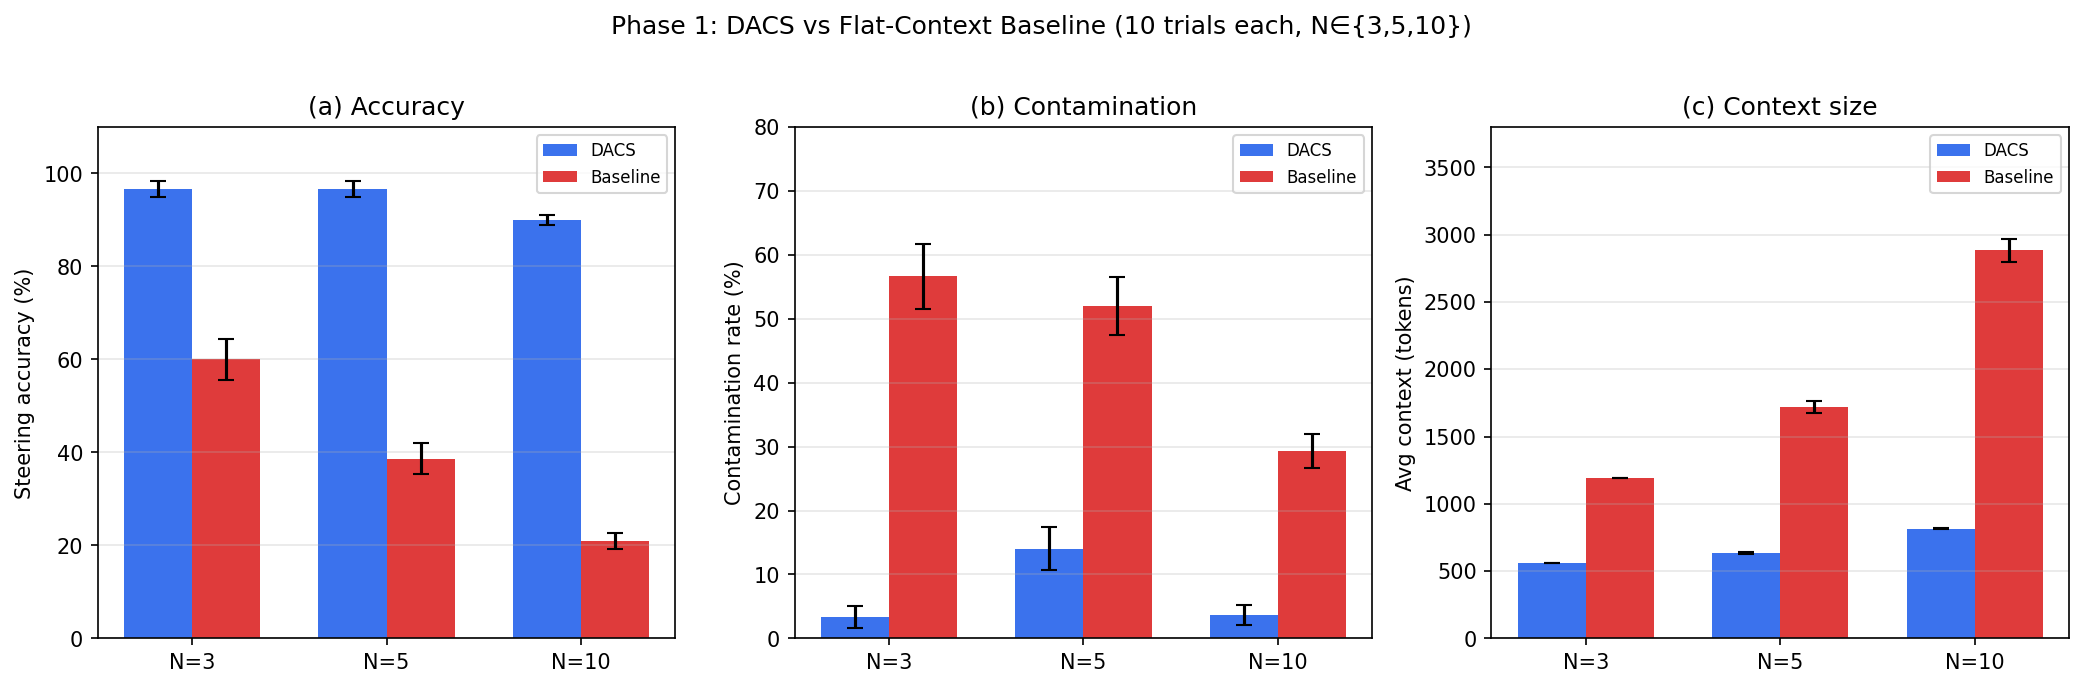
\includegraphics[width=\textwidth]{figures/phase1_overview.png}
  \caption{DACS vs.\ flat-context baseline across $N \in \{3,5,10\}$.
  Error bars: $\pm 1$ SE (10 trials each).
  (a) Steering accuracy.
  (b) Wrong-agent contamination.
  (c) Average context tokens at steering time.
  Context size annotations show the efficiency ratio $\rho(N)$.}
  \label{fig:overview}
\end{figure}

\subsection{Accuracy Gap Grows with $N$}

The DACS advantage is not constant across $N$—it grows monotonically.
At $N=3$ the gap is $+36.7$ pp; at $N=10$ it reaches $+69.0$ pp, with
baseline accuracy collapsing to 21\%.
This is the signature prediction of the context pollution hypothesis:
as more agent threads compete for a flat context window, the
orchestrator's ability to give correct, focused steering responses
degrades, while DACS's isolation guarantees maintain high accuracy.

\subsection{Sub-linear Context Scaling}
\label{sec:scaling}

DACS context at steering time grows from 561 ($N=3$) to 633 ($N=5$) to
816 ($N=10$) tokens.
A linear fit to $(N, |C_{\text{focus}}|)$ gives slope $\hat{\beta} = 25.5$
tokens/agent ($R^2 > 0.99$), exactly consistent with the theoretical
prediction of $\approx |r|$ tokens per additional agent.

Baseline context grows from 1{,}191 to 1{,}720 to 2{,}883 tokens.
The efficiency ratio $\rho(N)$ increases at every step: 2.12, 2.72,
3.53$\times$.
At the theoretical maximum ($N \to \infty$, $|F|/|r| \approx 20$), the
ratio would approach $\approx 20\times$; we are on this trajectory.

\subsection{Contamination Analysis}

DACS contamination at $N=3$ and $N=10$ is below 4\%—essentially zero.
The $N=5$ mean of 14\% is driven by a single trial (trial t03, 40\%
contamination); the median $N=5$ DACS contamination is 6.7\%.
Investigating trial t03, the steering response for the graph BFS/DFS agent
contained terminology that has moderate overlap with two other agents'
domains (graph structure terminology appears in both the BFS agent and
the RL policy gradient agent's domain).
This suggests that even with focus isolation, vocabulary coincidence
between conceptually adjacent agent domains can cause false-positive
contamination detections.
We treat keyword-based contamination scoring as a lower bound on true
isolation quality.

The baseline contamination pattern is notable: it decreases from 57\% to
52\% to 29\% as $N$ increases, opposite to what a naïve pollution model
would predict.
We hypothesise two mechanisms: (1) at high $N$, the requesting agent's
detailed, domain-specific question dominates the flat context, causing
the LLM to default to addressing that agent despite all other threads
being present; (2) at high $N$, the baseline routing prompt becomes more
structured (more agents to address forces a table-format response), which
accidentally improves precision.
Crucially, neither mechanism improves baseline \emph{accuracy}—baseline
accuracy degrades from 60\% to 21\% as $N$ grows, confirming that the
orchestrator still gives wrong answers even when it addresses the right
agent.

%-----------------------------------------------------------------------
\section{Discussion}
\label{sec:discussion}

\subsection{Why DACS Works}

The mechanism's effectiveness follows directly from what it removes from
the context window.
In the flat baseline, when $a_i$ asks ``should I use recursive or
iterative traversal for my BST inorder walk?'', the context simultaneously
holds a research agent's detailed transformer attention analysis and a
data processor's CSV encoding problem, containing domain keywords
(``attention'', ``heads'', ``encoding'', ``UTF-8'') that have nothing to
do with the correct answer.
The LLM anchors its response to whichever content pattern captures its
attention—an effect we measure as both inaccuracy and contamination.

DACS removes this anchor competition entirely.
In \textsc{Focus}$(a_i)$ mode, the context contains $a_i$'s task
description and steering history plus compact status lines for other
agents (``a2: RUNNING, transformer survey, 3/5 steps done'').
The correct-answer vocabulary dominates the context by construction.

\subsection{Relation to Hierarchical Routing}

DACS is orthogonal to hierarchical agent architectures
(AgentOrchestra~\citep{agentorchestra2025},
AdaptOrch~\citep{adaptorch2025b}).
Hierarchical routing reduces \emph{how many} agent threads reach the
orchestrator at all—it bounds the problem at task decomposition time.
DACS controls \emph{what} the orchestrator holds in its context at each
steering moment during execution.
A production system could combine both: hierarchical routing limits the
active agent pool, and DACS ensures that within that pool, each steering
interaction is clean.

\subsection{Limitations}

\paragraph{Benchmark scope.}
The task suite uses keyword matching to evaluate steering accuracy.
This is conservative (multi-word phrases and paraphrases are not captured)
and may produce false-positive contamination detections when domains share
vocabulary.
A more robust evaluation would use LLM-as-judge scoring or a task suite
with guaranteed vocabulary disjointness.

\paragraph{Synthetic agents.}
Our agent stubs simulate decision points with pre-defined timing and
question templates.
Real agents have irregular steering request patterns, potentially large
partial outputs, and multi-turn steering histories.
We expect DACS's context efficiency advantage to be larger in practice
(more tokens in $F(a_i)$), but accuracy effects depend on the actual
complexity of real-world decision points.

\paragraph{Single model and context budget.}
All experiments use MiniMax-M2.7 at a 204{,}800-token budget.
With a smaller budget (e.g., 8{,}192 tokens), context pollution effects
would be more severe and DACS's advantage even larger.
With very large budgets, the flat baseline may degrade less at moderate
$N$.
Results may differ across model families with different attention
characteristics.

\paragraph{Interrupt handling not experimentally isolated.}
The interrupt protocol (transition~\eqref{eq:t3}) was exercised naturally in
experiments but not ablated independently.
An ablation isolating interrupt frequency and its effect on accuracy would
strengthen the mechanistic account.

\subsection{Future Work}

Immediate extensions:
\begin{itemize}
  \item \textbf{User responsiveness.} Measure the latency from user
  message to orchestrator response under DACS vs.\ baseline at varying
  $N$ and steering queue depth.
  \item \textbf{Interrupt ablation.} Vary the \textsc{High}-urgency
  threshold and measure the accuracy-latency tradeoff.
  \item \textbf{Long-horizon tasks.} Run agents with multi-turn steering
  histories (5+ exchanges per agent) to stress-test focus context size
  bounds.
  \item \textbf{Real application integration.} Integrate DACS as a
  drop-in context management layer in an existing production multi-agent
  system (e.g., as a wrapper around an AgentOrchestra-style planner).
\end{itemize}

%-----------------------------------------------------------------------
\section{Conclusion}
\label{sec:conclusion}

We presented DACS, a dynamic attentional context scoping mechanism that
solves context pollution in multi-agent LLM orchestration through
agent-triggered asymmetric focus sessions.
The mechanism is exact (not approximate), sub-linear in agent count, and
fully compatible with existing orchestration architectures.
Across 60 experimental trials, DACS achieves $+36.7$ to $+69.0$ pp
steering accuracy improvement over a flat-context baseline, reduces
wrong-agent contamination from $29$--$57\%$ to $4$--$14\%$, and
exhibits a growing context efficiency advantage (2.12--3.53$\times$) as
$N$ increases from 3 to 10.

The core contribution is demonstrating that \emph{what is in the
orchestrator's context window at the moment of steering} is the
dominant variable for multi-agent steering accuracy—not model size,
not topology, not memory compression—and that a simple, deterministic
mode-switch mechanism suffices to control it effectively.

%-----------------------------------------------------------------------
\bibliographystyle{plainnat}
\bibliography{refs}

\end{document}
